
\subsection{Power Supply}

The power supply on the segway was designed to deliver 5V to the FPGA.
The PCB was constructed such that it also featured the connectors needed such that the FPGA, IMU, bluetooth and wheel encoders could be directly plugged into the board.


\begin{figure}[H]
\centering 
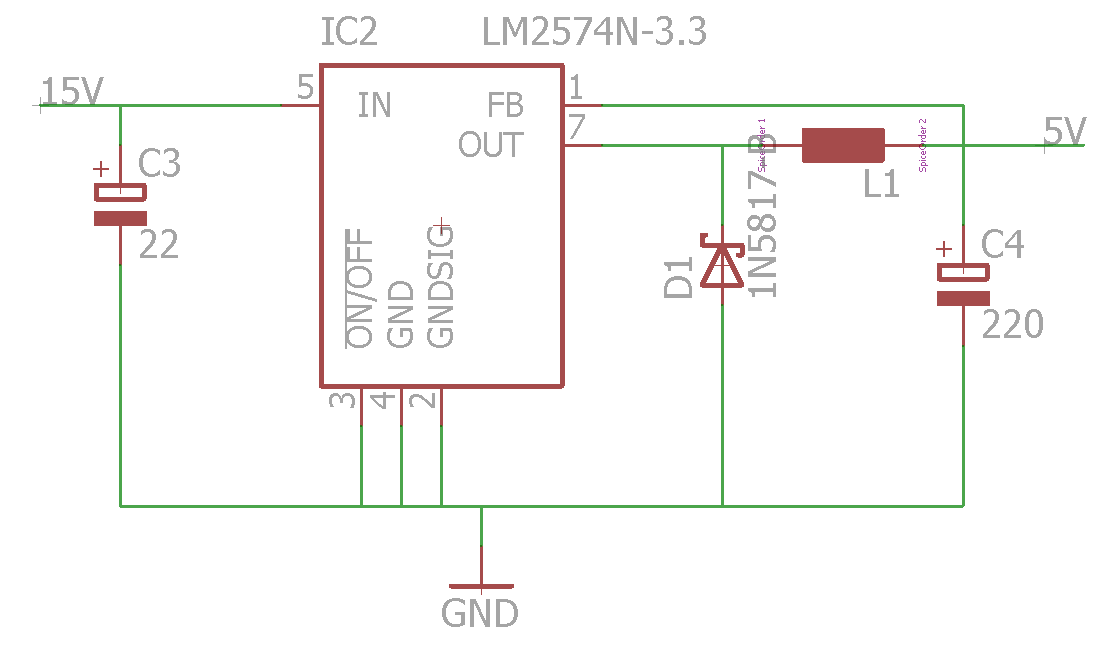
\includegraphics[width = 0.5 \textwidth]{images/powersupply}
\caption{Schematics of the power supply.}
\label{fig:powersupply_schematics}
\end{figure}

To ensure a 5V/0.5A supply for the FPGA an LM2574 switching regulator is used. 
The advantage of using a switching regulator on the segway is that the efficiency of switching regulators is higher than that of linear regulators.
This maximizes the power efficiency of the device, which is useful if it has to drive on battery.

Furthermore the efficiency of the 5V power supply was calculated.
This was done using equation \ref{eq:powersupply_efficiency}.

\begin{equation}
Efficiency = \frac{P_{out}}{P_{in}} = \frac{V_{out}^2 / R_{out}}{V_{in} \cdot I_{in}}
\label{eq:powersupply_efficiency}
\end{equation}

Where, in equation \ref{eq:powersupply_efficiency}, V is the voltage (V), R the resistance added ($\Omega$) and I the current (A) for the circuit where \textit{in} is what was supplied by the 15V supply used for testing and \textit{out} the output of the regulator.


\begin{table}[H]
\centering
\begin{tabular}{|c|c|c|c|c|}
\hline
Load ($A$) & Min Efficiency & Avg. Efficiency & Max Efficiency \\ \hline
1.00 & 0.7806 & 0.7996 & 0.8367 \\ \hline
0.67 & 0.7570 & 0.8095 & 0.8096 \\ \hline
0.33 & 0.7556 & 0.7640 & 0.8587 \\ \hline
0.15 & 0.644 & 0.6607 & 0.7318 \\ \hline
\end{tabular}
\caption{Efficiency of the 5V supply.}
\label{tab:voltageefficiency}
\end{table}

The efficiency was calculated considering that the input supply is stable and using the maximum, minimum and average output voltages measured with the oscilloscope.
It can be seen from table \ref{eq:powersupply_efficiency} that as the load decreases to less than $0.67A$ the efficiency decreases considerably.
This is however expectable since the regulator used specifies that the efficiency is highest when driving a load with 0.5A at 5V and then only is specified to achieve an 80\% efficiency.

Since the motors are specified to drive at 200mA, then it is expected that the full system consumes around 0.5A when running.
This should hence yield on average a good efficiency of the energy consumption while it is still possible for the motors to pull combined up to, and possibly above, 1A if needed.


